\documentclass[12pt]{article}

\usepackage[margin=1.0in]{geometry}
\usepackage{tabto}
\usepackage{amsmath}
\usepackage{framed}
\usepackage{graphicx}
\usepackage{listings}
\usepackage{color} %red, green, blue, yellow, cyan, magenta, black, white
\definecolor{mygreen}{RGB}{28,172,0} % color values Red, Green, Blue
\definecolor{mylilas}{RGB}{170,55,241}
\graphicspath{ {./} }

\newcommand*\lstinputpath[1]{\lstset{inputpath=#1}}



\begin{document}

\title{CS / MATH 4334 : Numerical Analysis\\Homework Assignment 4}
\author{Matthew McMillian\\mgm160130@utdallas.edu}
\maketitle

\section*{MatLab Problems}

\lstset{language=Matlab,%
    %basicstyle=\color{red},
    breaklines=true,%
    morekeywords={matlab2tikz},
    morekeywords=[2]{1}, keywordstyle=[2]{\color{black}},
    identifierstyle=\color{black},%
    showstringspaces=false,%without this there will be a symbol in the places where there is a space
    numbers=left,%
    numberstyle={\tiny \color{black}},% size of the numbers
    numbersep=9pt, % this defines how far the numbers are from the text
    emph=[1]{for,end,break},emphstyle=[1]\color{red}, %some words to emphasise
    %emph=[2]{word1,word2}, emphstyle=[2]{style},    
}

\pagebreak

	\begin{enumerate}
	
	\item[] Problem 1 : q1.m \noindent\rule{\textwidth}{1.0pt} \\
	\lstinputlisting{q1.m}	
	
	\pagebreak	
	
	$>>$ q1.m
	\begin{framed}
		ans =\\

    'We notice that as h gets smaller, the error decreases. However, due to a combonation of truncation, roundoff errors and loss of signifigance we see weird behavious from h as it gets smaller and smaller. Our h value that we got was close our expected h value form problem 2.'

	\end{framed}
	
	\begin{center}
		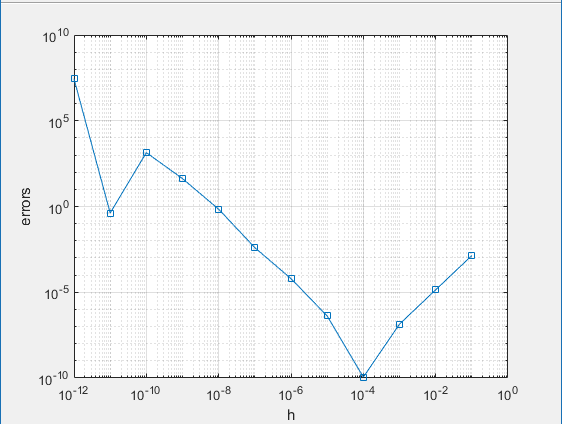
\includegraphics[scale=0.95]{graph1}
	\end{center} 
	
	\end{enumerate}
	\pagebreak	
	
	\begin{enumerate}
	
	\item[] Problem 2 : q2.m \noindent\rule{\textwidth}{1.0pt} \\
	\lstinputlisting{q2.m}
	
	\item[] Problem 2 : trapfun.m \noindent\rule{\textwidth}{1.0pt} \\
	\lstinputlisting{trapfun.m}	
	
	\item[] Problem 2 : simpfun.m \noindent\rule{\textwidth}{1.0pt} \\
	\lstinputlisting{simpfun.m}	
	
	\pagebreak	
	
	$>>$ q2.m
	\begin{framed}
		ans =\\
     9.640822025822844e+01\\


ans =\\
     9.640696765218401e+01\\


ans =\\
    'a) 96.41 students would fail this class based on trapezoid rule.\\
     b) 96.41 students would fail based on simpsons rule.\\
     No, we definitely would not want to take this class'
	\end{framed}
	
	\end{enumerate}
	\pagebreak
	\begin{enumerate}
	
	\item[] Problem 3 : q3.m \noindent\rule{\textwidth}{1.0pt} \\
	\lstinputlisting{q3.m}
	
	\item[] Problem 3 : rombergmod.m \noindent\rule{\textwidth}{1.0pt} \\
	\lstinputlisting{rombergmod.m}	
	
	
	\pagebreak	
	
	$>>$ q3.m
	\begin{framed}
	There are 129 function evals, and the approximation is of order 16. \\
		\begin{center}
			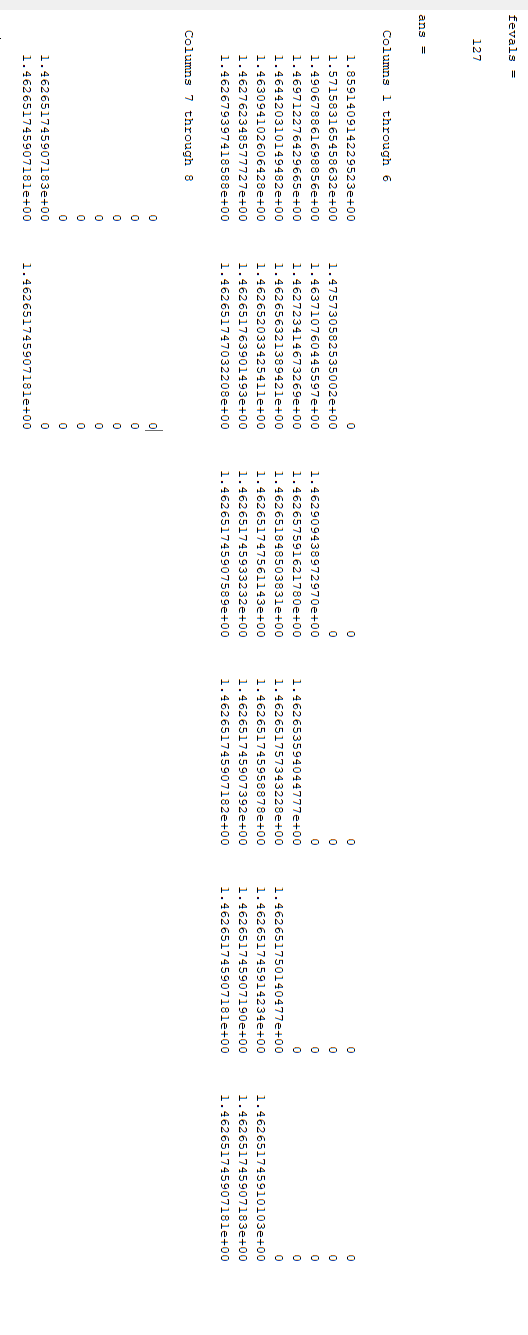
\includegraphics[scale=0.55]{q3out2}
		\end{center} 
	\end{framed}
	
	\end{enumerate}
	
	
	
\end{document}